\section{Response of First Order Circuits}

\subsection{The Step Response of RC and RL Circuits}
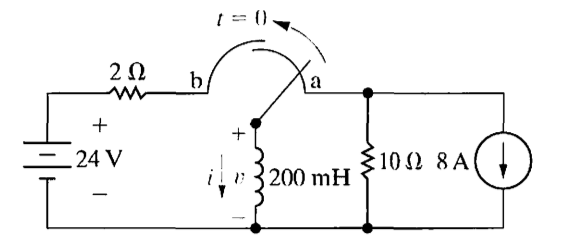
\includegraphics[scale=0.5]{img/c7/p1}

Assume that the switch in the circuit shown in the figure above has been in position b for a long
time, and at $t = 0$ it moves to position a. Find:

\begin{enumerate}
	\item $i(0^{+}$
	\item $ v(0^{+}) $
	\item $ \tau, t > 0 $
	\item $i(t), t \geq 0$
	\item $v(t), t \geq 0^{+}$
\end{enumerate}

We begin my solving for $i(0^{+})$:\\
Using the circuit shown below at t < 0, we can calculate the initial current 
in the inductor. \\
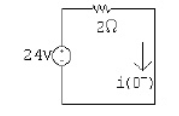
\includegraphics{img/c7/a1} \\	
We can solve for the current at time $i(0^{-})$ because the current in an
inductor is continuous.
\\ $i(0^{-} = \frac{24}{2} = 12 A = i(0^{+}) $ \\
Next, using the current at $t = 0^{+}$, as shown below, we can calculate the
voltage drop across the inductor at $0^{+}$. Note that this is the same as the
voltage drop across the $10\Omega$ resistor, which has current from two sources,
8A from the current source and 12 A from the initial current through the
inductor. \\
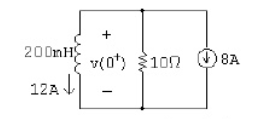
\includegraphics{img/c7/a2}\\
$ v(0^{+}) = -10(8+12) = -200 V $ \\
Now, to calculate the time constant we need the equivalent resistance seen
by the inductor for $t > 0 $. Only the $10 \Omega$ resistor is connected to
the inductor for $ t > 0$. Therefore:
\\ $ \tau = \frac{L}{R} = \frac{200 \time 10^{-3}}{10} = 20 ms $ \\

Then, to find $i(t)$ we need to find the final value of the current in the
inductor. When the switch has been in position a for a long time, the circuit
reduces to the one below:\\
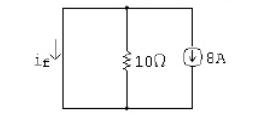
\includegraphics{img/c7/a3}\\
Its important to notice that the inductor behaves like a short circuit and all
of the current from the 8 A source flows through the short circuit. Thus: \\
$ i_f = -8 A $ \\
Therefore:
\begin{align*}
	i(t) &= i_f + [i(0^{+}) - i_f]e^{\frac{-t}{\tau}} \\
	i(t) &= -8 + [12 - (-8)]e^{\frac{-t}{0.02}} \\
	i(t) &= -8 + 20e^{-50t} A, t \geq 0 \\
\end{align*}
Finally, to find $v(t)$, we can use the relationship between voltage and 
current for an inductor:
\begin{align*}
	v(t) &= L\frac{di(t)}{dt} \\
	v(t) &= (200 \times 10^{-3})(-50)(20e^{-50t}) \\
	v(t) &= -200e^{-50t} V, t \geq 0^{+} \\
\end{align*}



\subsection{Sequential Switching}
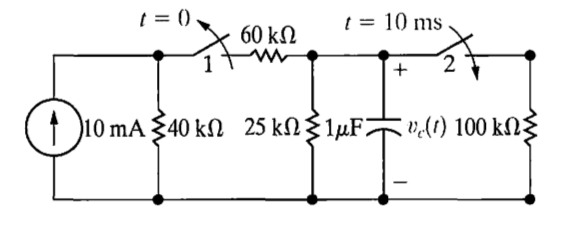
\includegraphics[scale=0.5]{img/c7/p2}

In the circuit shown, switch 1 has been closed and switch 2 has been open for a long time. At t=0,
switch 1 is opened. Then 10 ms later, switch 2 is closed. Find:

\begin{enumerate}
	\item $v_c(t) for 0 \leq t \leq 0.01$ s
	\item $v_c(t) for t \geq 0.01$ s
	\item the total energy dissipated in the $25 k\Omega$ resistor
	\item the total energy dissipated in the $100 k\Omega$ resistor
\end{enumerate}

1) Use the circuit shown below, for $t < 0$, to calculate the initial
voltage drop across the capacitor:\\
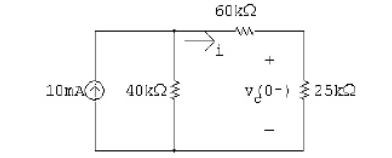
\includegraphics{img/c7/a21} \\
\\ $ i = \left(\frac{40 \times 10^{3}}{125 \times 10^{3}} \right)(10 \times 10^{-3} = 3.2 mA $ \\
\\ $v_c(0^{-} = (3.2 \times 10^{-3})(25 \times 10^{3}) = 80 V = v_c(0^{+})$ \\
Now we ca use the following circuit, valid for $0 \leq t \leq 10 ms$ to 
calculate $v_c(t)$ for that interval: \\
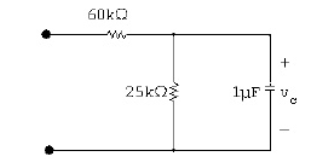
\includegraphics{img/c7/a22} \\
For $0 \leq t \leq 100 ms$: 
\begin{align*}
	\tau &= RC \\
	\tau &= (25 \times 10^3)(1 \times 10^{-6}) \\
	\tau &= 25 ms \\
	v_c(t) &= v_c(0^{-})e^{\frac{t}{\tau}} \\
	&= 80e^{-40t} V, 0 \leq t \leq 10ms \\	
\end{align*}
2) Now we can calculate the starting capacitor voltage in the interval 
$t \geq 10 ms$, to calculate $v_c(t)$ for that interval: \\
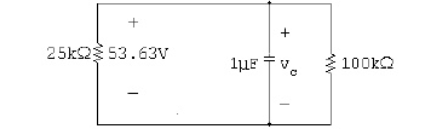
\includegraphics{img/c7/a23} \\
For $t \geq 10 ms$: \\
$R_{eq} = 25 k\Omega \parallel 100k\Omega = 20k\Omega $ \\
$ \tau = R_{eq}C = (20 \times 10^{3})(1 \times 10^{-6}) = 0.02 s $\\
Therefore:
\begin{align*}
	v_c(t) &= v_c(0.01^{+})e^{-(t-0.02)/\tau} \\
	&= 53.63e^{-50(t-0.01)} V, t \geq 0.01 s \\
\end{align*}
3) To calculate the energy disiated in the $25 k\Omega$ resistor, we can
integrate the power absorbed by the resistor over all time. Use
the expression $p = v^2/R$ to calculate the power absorbed. 
\begin{align*}
	w_{25k} &= \int{0}^{0.01} \frac{[80e^{40t}]^2}{25000}dt + \int{0.01}^{\infty} \frac{[53.53e^-50(t-0.01)]^2}{25000} dt \\
	w_{25k} &== 2.91 mJ \\
\end{align*}

4) We can repeat the process from (3), but keeping in mind that the voltage
across this resistor is non-zero only for the second interval:
\begin{align*}
	w_{100k\Omega}  &= \int{0.01}{\infty} \frac{[53.63e^{-50(t-0.01)}]^2}{100000} dt \\
	w_{100k\Omega} &= 0.29 mJ \\
\end{align*}


